\chapter{线程}
\label{chap:thread}

\section{线程基础知识}

\subsection{线程状态}

JVM线程的状态定义在Thread.State枚举中。包括:

\begin{itemize}
    \item   NEW         新建
    \item   RUNNABLE    就绪
    \item   BLOCKED     阻塞 
    \item   WAITING     
    \item   TIMED\_WAITING
    \item   TERMINATED
\end{itemize}


\begin{figure}[H]
    \centering
    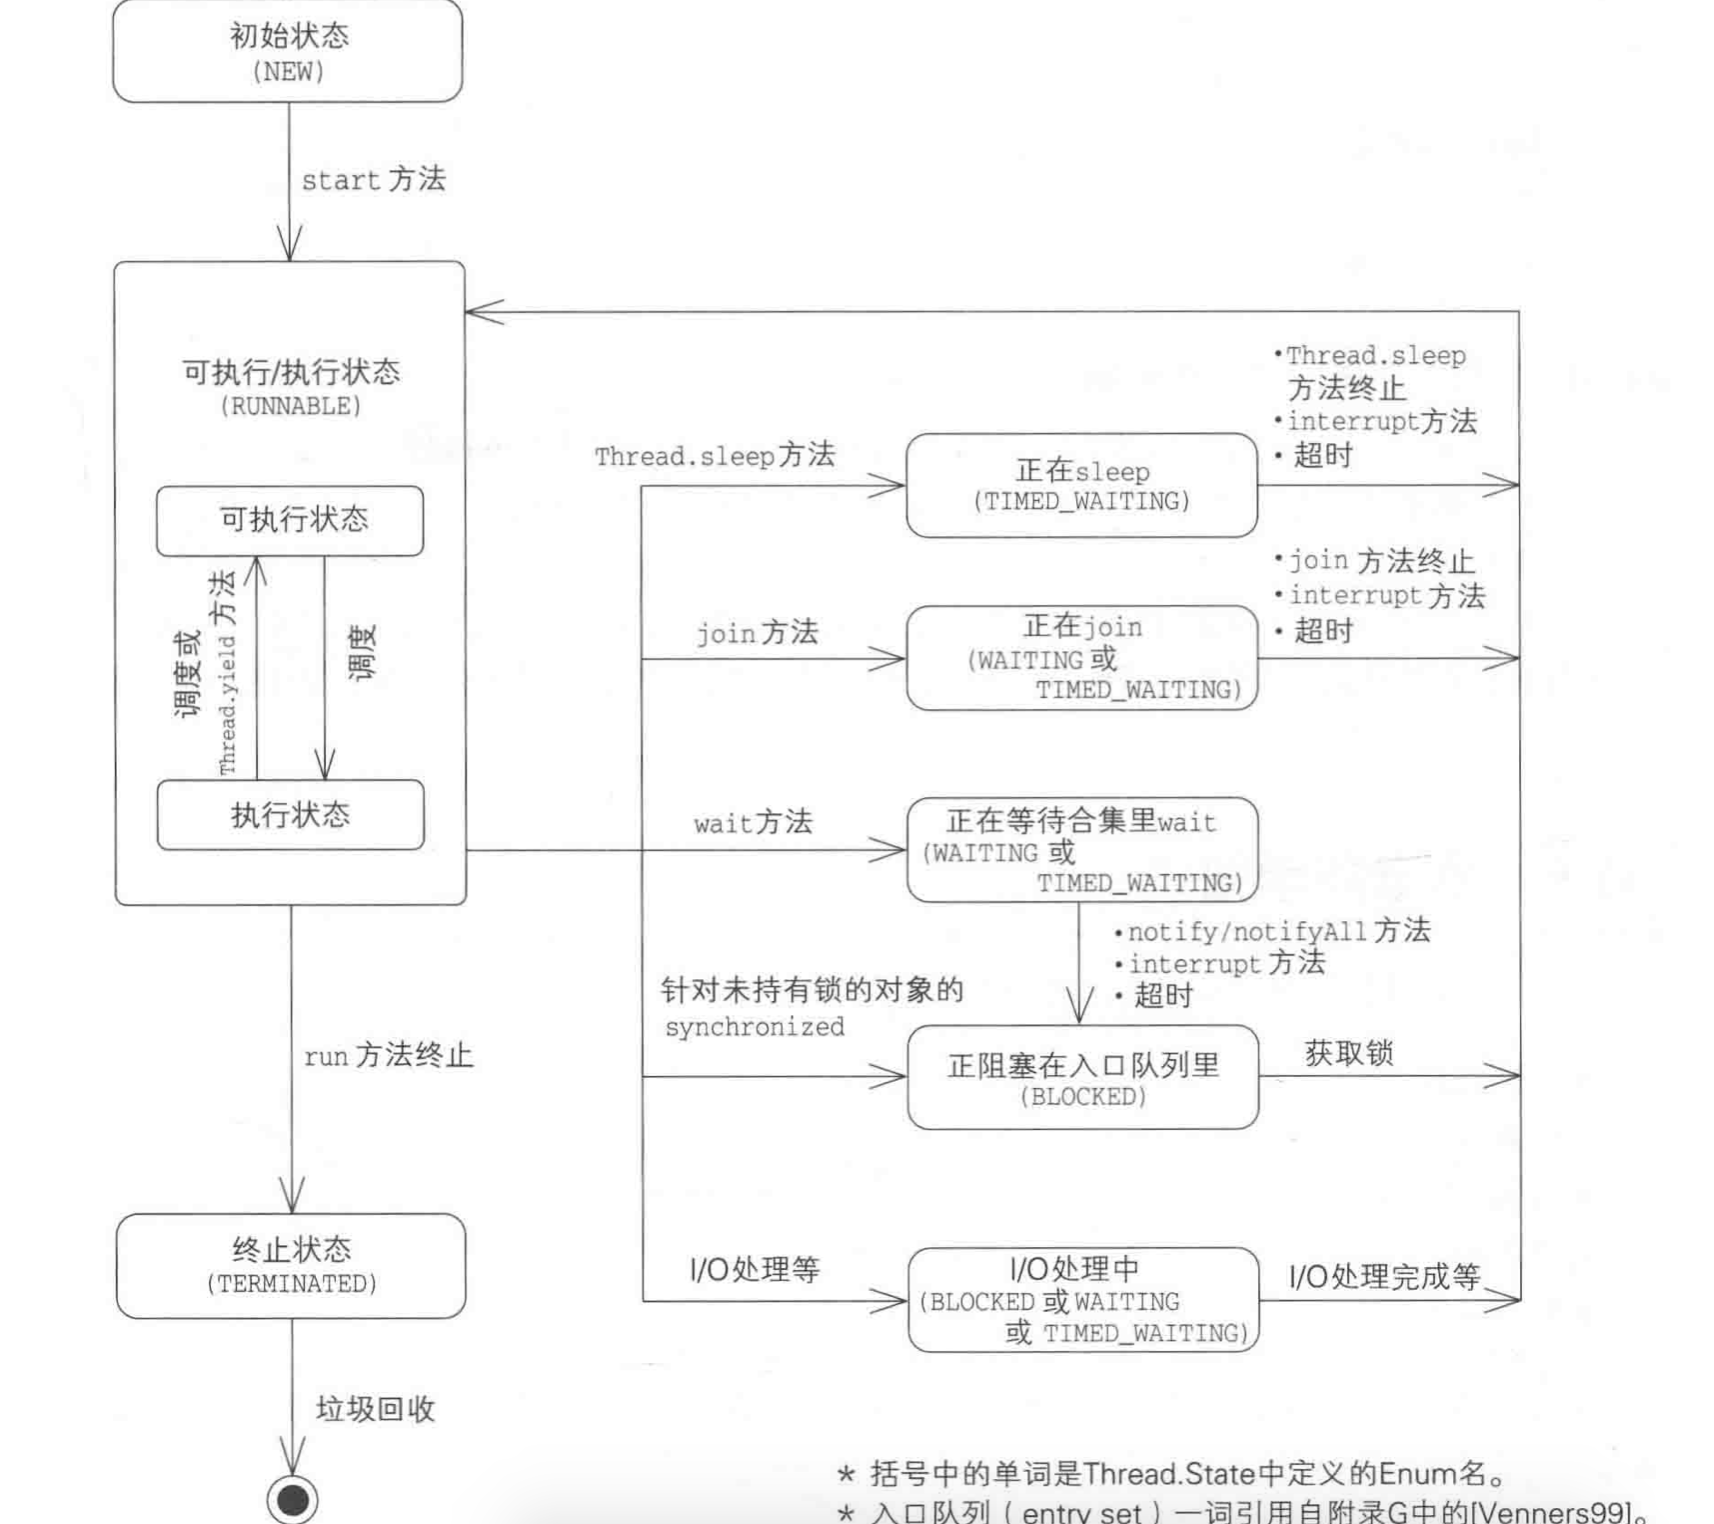
\includegraphics[width=1\textwidth]{thread/thread_states.png}
    \caption{线程状态迁移图(摘自《图解Java多线程设计模式》)}
\end{figure}

\subsubsection{NEW}

当线程被创建时,它只会短暂地处于这种状态。此时它已经分配了必须的系统资源,并执行了初始化。


\subsubsection{RUNNABLE}

只要调度器把时间片分配给线程,线程就可以运行。



下面为State枚举


\begin{lstlisting}[language=java]

public enum State {
        /**
         * 尚未启动的线程的线程状态
         */
        NEW,

        /**
         * 可运行线程的线程状态。 处于可运行状态的线程正在Java虚拟机中执行,
         * 但是它可能正在等待来自操作系统(例如处理器)的其他资源。
         */
        RUNNABLE,

        /**
         * 线程的阻塞状态,等待监视器锁定。
         * 处于阻塞状态的线程正在等待一个监视器锁进入一个同步块/方法,
         * 或者在调用Object.wait()后重新进入一个同步块/方法。
         */
        BLOCKED,

        /**
         * 等待线程状态
         * 一个线程由于调用下列方法之一而处于等待状态:
         * 
         *   Object.wait() 未超时
         *   Thread.join() 未超时
         *   LockSupport.park()
         * 
         * 处于等待状态的线程正在等待另一个线程执行特定的操作。
         * 例如: 一个线程在一个对象上已经调用了 Object.wait() ,并正在等待在另一个线程在另一对象上调用
         * Object.notify() or Object.notifyAll()。
         * 调用 thread.join() 的线程正在等待指定的线程终止。
         */
        WAITING,

        /**
         * 具有指定等待时间的等待线程的线程状态。
         * 线程处于定时等待状态,因为调用以下方法之一与指定的正等待时间:
         * 
         *   Thread.sleep()
         *   Object.wait(long)带超时参数
         *   Thread.join(long)带超时参数
         *   LockSupport.parkNanos
         *   LockSupport.parkUntil
         * 
         */
        TIMED_WAITING,

        /**
         * 终止状态。线程已经完成执行。
         */
        TERMINATED;
    }

\end{lstlisting}


\subsection{创建线程的方式}

创建线程的根本方法就是通过构造Thread类并且重写run()方法,然后调用start方法运行。

\begin{lstlisting}[language=java]

    public Thread();
    public Thread(String name);
    public Thread(ThreadGroup group, String name);

    public Thread(Runnable target);
    public Thread(Runnable target, String name);
    public Thread(ThreadGroup group, Runnable target, String name);
    public Thread(ThreadGroup group, Runnable target, String name, long stackSize);

\end{lstlisting}


创建线程有四种方式

\begin{itemize}
    \item  继承Thread类 
    \item  实现Runnable接口
    \item  实现Callable和Future接口
    \item  使用线程池方式
\end{itemize}


\subsubsection{实现Runnable接口}

Runnable接口

\begin{lstlisting}[language=java]

    @FunctionalInterface
    public interface Runnable {
        public abstract void run();
    }

\end{lstlisting}

\begin{lstlisting}[language=java]

public class HelloRunnable implements Runnable {

    public void run() {
        System.out.println("Hello from a thread!");
    }

    public static void main(String args[]) {
        (new Thread(new HelloRunnable())).start();
    }
}

\end{lstlisting}

\subsubsection{继承Thread类}

Thread类也继承了Runnable接口

\begin{lstlisting}[language=java]

    public class MyThread extends Thread {
        public void run() {
            System.out.println(Thread.currentThread().getName() + ": Run!!!");
        }
    
        public static void main(String[] args) {
            MyThread thread = new MyThread();
            thread.start();
        }
    }

\end{lstlisting}

\subsubsection{实现Callable和Future接口}

\begin{figure}[H]
    \centering
    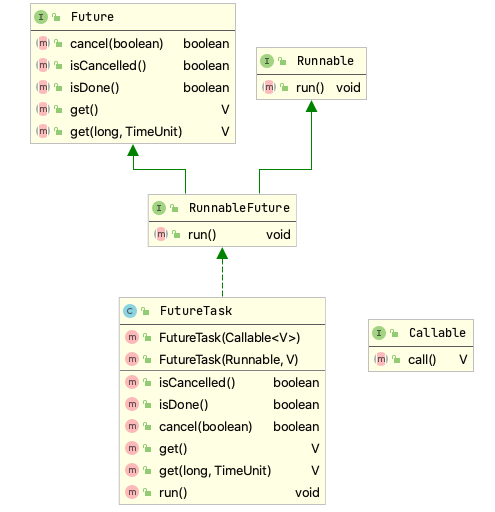
\includegraphics[width=0.8\textwidth]{thread/futuretask_diagram.png}
\end{figure}


\begin{lstlisting}[language=java]
    public class TaskWithResult implements Callable {

        private int id;
        public TaskWithResult(int id) {
            this.id = id;
        }

        @Override
        public Object call() throws Exception {
            return "Result of TaskWithResult is: " + id;
        }
    }

    public class FutureAndCallable {
    public static void main(String[] args) throws ExecutionException, InterruptedException {
        //不推荐使用Executors
        ExecutorService executorService = Executors.newCachedThreadPool();
        List<Future<String>> result = new ArrayList<>();
        for (int i = 0; i < 10; i++) {
            result.add(executorService.submit(new TaskWithResult(i)));
        }

        for (Future<String> future : result) {
            System.out.println(future.get());
        }

        executorService.shutdown();
    }
}



\end{lstlisting}


\subsubsection{使用线程池方式}

\begin{figure}[H]
    \centering
    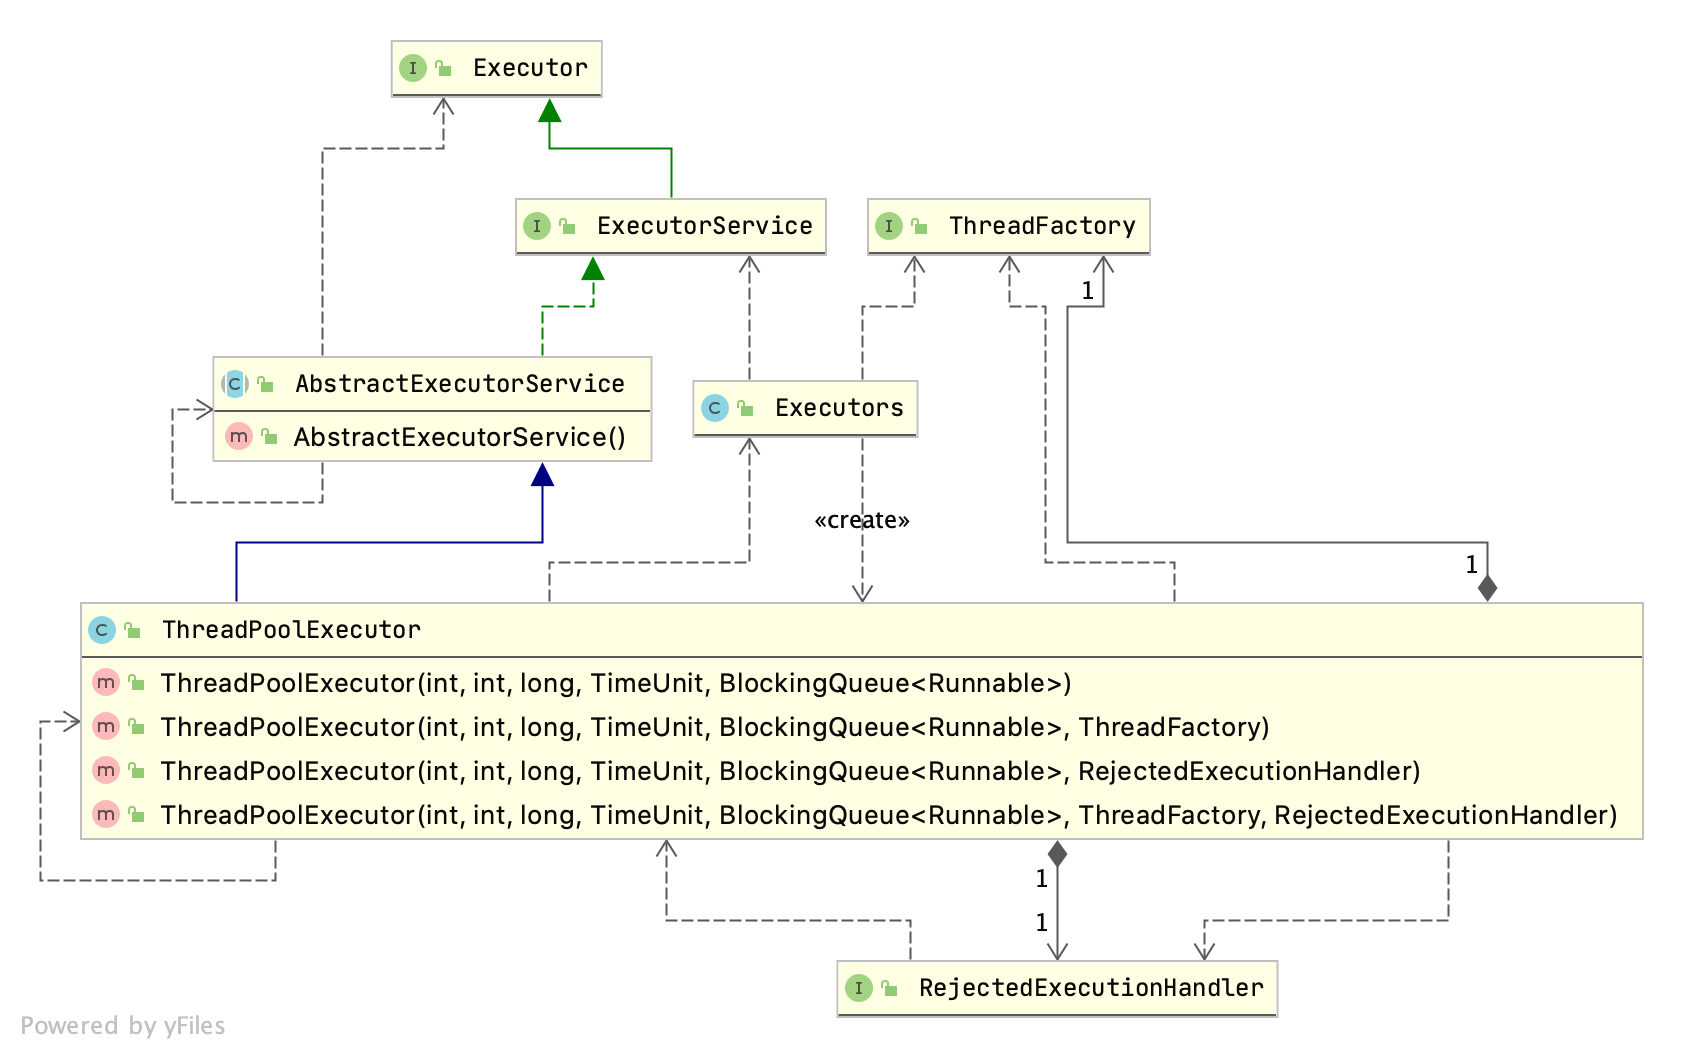
\includegraphics[width=1\textwidth]{thread/executor_diagram.png}
\end{figure}

线程池不允许使用 Executors 去创建,而是通过 ThreadPoolExecutor 的方式,这样的处理方式让写的同学更加明确线程池的运行规则,规避资源耗尽的风险。

Executors提供了如下线程池

\begin{itemize}
    \item newSingleThreadExecutor
    \item newFixedThreadPool
    \item newCachedThreadPool
    \item newScheduledThreadPool
    \item newSingleThreadScheduledExecutor
    \item newWorkStealingPool
\end{itemize}

\notebox{
    FixedThreadPool和SingleThreadExecutor:\newline
    运行的请求队列长度为Integer.MAX\_VALUE,可能会堆积大量的请求,从而导致OOM。

    CachedThreadPool:\newline
    允许的创建线程数为Integer.MAX\_VALUE,可能会创建大量的线程,从而导致OOM。
}

\begin{lstlisting}[language=java]
// 不推荐
ExecutorService executorService = Executors.newCachedThreadPool();

for (int i = 0; i < 5; i++) {
    executorService.execute(()->{
        System.out.println("Hello from a thread!");
    });
}

executorService.shutdown();

//推荐;指定最大线程数以及列队数
ExecutorService executor = new ThreadPoolExecutor(5, 5, 10L, TimeUnit.MILLISECONDS, new LinkedBlockingQueue<>(10));
for (int i = 0; i < 10; i++) {
    executor.execute(() -> System.out.println(Thread.currentThread().getName() + ":ThreadPoolExecutor"));
}

executor.shutdown();

\end{lstlisting}


\subsection{捕获异常}

不能捕获从线程中逃逸的异常。一旦异常跳出任务的run()方法,它就会向外传播到控制台。

可通过重写UncaughtExceptionHandler实现。使用setUncaughtExceptionHandler或者setDefaultUncaughtExceptionHandler方法。



\subsection{常用函数}

\begin{itemize}
    \item wait
    \item sleep
    \item join
    \item yield
    \item notify
    \item notifyAll
    \item interrupt
\end{itemize}


\subsubsection{wait}
调用wait()会释放对象上的锁。 

wait() 有两种形式。

第一种接受毫秒数做为参数,指“在此期间暂停”

在wait()期间对象锁是释放的
可以通过notify(),notifyAll()或者令时间到期,从wait()中恢复执行。

第二种不接受任何参数

wait()无限等待下去,直到线程接收到notify()或者notifyAll()的消息。

\subsubsection{sleep}
 调用sleep()的时候锁并不会被释放。

 \subsubsection{yield}
 yield()的时候锁并不会被释放。

\subsubsection{join}


wait(),notify(),notifyAll()是基类Object的一部分,而不是属于Thread的一部分。
只能在同步控制方法或者同步控制块里调用这三个方法,调用他们必须获取对象的锁。

为防止错失信号

\begin{lstlisting}[language=java]

    synchronized(sharedMonitor){
        while(someCondition){
            shareMonitor.wait();
        }
    }

\end{lstlisting}



\subsection{终止}

I/O和在synchronized块上的等待是不可中断的。













